\documentclass[11pt]{article}

\usepackage[utf8]{inputenc}
\usepackage[T1]{fontenc}
\usepackage{lmodern}
\usepackage[margin=2.5cm]{geometry}
\usepackage{amsmath}
\usepackage{booktabs}
\usepackage{graphicx}
% hyperref needs letltxmacro.sty (texlive-latex-extra); skipped when it is not installed.
\IfFileExists{letltxmacro.sty}{\usepackage{hyperref}}{}
\usepackage[numbers]{natbib}

\title{Small Models that Forget: Exploiting Temporal Locality\\ with Online Learning at Inference Time}
\author{Ruben Tous\\ \small{\textit{Affiliation}}}
\date{Draft, \today}

\begin{document}
\maketitle

\begin{abstract}
Many inputs that machine learning models see at inference time have strong temporal locality:
consecutive inputs tend to be similar and come from a small part of the input distribution.
A model facing such inputs does not need to keep everything it knows ready at all times.
It may be enough to remember some basic knowledge and adapt quickly to the current context.
We study whether this allows smaller models.
Neural networks of decreasing size are trained offline on MNIST and then updated online, one image at a time, while they classify a stream of test images arranged in bursts of three digits.
A shuffled copy of the same stream serves as a control without locality.
With plain SGD, small multilayer perceptrons trained online classify the bursty stream more accurately than their frozen offline version, and the gain over the shuffled stream grows as the model shrinks and as the online learning rate increases.
For the smallest model (6.2\,KB), online learning raises accuracy from 64.3\% to 70.7\%, while the same procedure on the shuffled stream lowers it to 63.7\%.
A small convolutional network also shows a locality effect, but with the single online learning rate tested it does not become more accurate than its frozen version.
\end{abstract}

\section{Introduction}

A trained network is usually deployed frozen: it must classify any input from the whole distribution it was trained on.
In many applications, however, the inputs arrive in a stream with strong temporal locality.
A camera in a kitchen sees kitchen objects for hours; a speech recognizer hears the same speaker for a whole conversation; a sensor stays in the same regime for long periods.
At any moment only a small part of the input distribution is active.

Computer memory hierarchies have relied on this property for decades: a small cache that holds the recently used data serves most requests \cite{denning1968working}.
We ask whether the same idea applies to the knowledge stored in a network.
A model does not need to remember everything all the time if its inputs have strong temporal locality.
It may only need some basic knowledge plus the ability to adapt fast to the current context.

Our hypothesis is that, under severe capacity limits, online training at inference time can outperform the same model trained offline and then frozen.
A frozen small model must spread its limited capacity over the whole distribution.
An online model can spend it on the part of the distribution that is active now.
The price is forgetting: neural networks trained sequentially lose what they learned earlier, a behavior known as catastrophic forgetting \cite{mccloskey1989catastrophic,french1999catastrophic}.
This recency bias is usually treated as a problem.
In a stream with temporal locality it may be useful, because what was seen recently is what will be seen next.

This paper reports a first set of experiments on MNIST \cite{lecun1998gradient}.
Experiment~1 checks whether small networks exploit temporal locality when they are simply trained online.
Experiment~2 explores whether a more aggressive online learning rate exploits it better.
Experiment~3 repeats the test with a small convolutional network.

\section{Related work}

\paragraph{Catastrophic forgetting and continual learning.}
Continual learning tries to learn a sequence of tasks without forgetting the earlier ones \cite{parisi2019continual,kirkpatrick2017overcoming}.
Our setting reverses the goal: we accept forgetting and ask whether it can be used.

\paragraph{Test time adaptation.}
Several methods update a model while it is used, for example with a self supervised task \cite{sun2020test} or by minimizing the entropy of the predictions \cite{wang2021tent}.
They target distribution shift and do not use labels.
Dynamic evaluation \cite{krause2018dynamic} updates a language model on the recent part of the sequence it is predicting, which exploits local regularities in text, the closest idea to ours.
Fast weights \cite{ba2016using} store recent information in weights that change quickly during inference.

\paragraph{Model compression.}
Compression reduces model size by pruning, quantization or distillation \cite{han2016deep}, keeping the model frozen.
We study a different route to small models that is complementary to compression.

\section{Method}

\subsection{Input streams}

The stream contains 10{,}000 positions built from MNIST test images.
It is divided into 193 bursts of random length between 10 and 95 images (51.8 on average).
Each burst picks 3 distinct digits at random, and every position in the burst is a random test image of one of those digits, drawn with replacement.
The stream holds 6{,}322 distinct test images.
As a reference for how much locality the stream has, predicting the label of the previous image is correct 32.3\% of the time.

The control stream is a random permutation of the same positions.
It contains exactly the same images, so any difference in accuracy comes from their order.
On the control stream, predicting the previous label is correct 9.9\% of the time.

\subsection{Protocol}

Each model is first trained offline on the 60{,}000 MNIST training images.
We call this the frozen model.
Then it processes a stream one image at a time.
For each image, the model first predicts its label, and the prediction counts towards the online accuracy.
Then it takes one optimization step on that single image with its true label.
This assumes that the label becomes available after each prediction, as in prequential evaluation.
Each stream starts from the same frozen weights.

We report four quantities, all on the same 10{,}000 positions:
\begin{itemize}
  \item \emph{frozen accuracy}: the frozen model without updates (equal on both streams, since they hold the same images);
  \item \emph{online accuracy on bursts} and \emph{online accuracy on random}: the online model on each stream;
  \item \emph{online gain}: online accuracy on bursts minus frozen accuracy;
  \item \emph{locality effect}: online accuracy on bursts minus online accuracy on random.
\end{itemize}
Differences are given in percentage points (pp).
The online gain tells whether online learning is worth it on the bursty stream.
The locality effect isolates the part of the gain that comes from temporal locality.
It removes the effect of simply training more, and of seeing some test images more than once, which happens in both streams.

Model size is the memory needed to store all parameters and buffers as 32 bit floats.
All runs use a fixed seed (0).

\subsection{Models}

The multilayer perceptron (MLP) has one hidden layer with ReLU: $784 \rightarrow h \rightarrow 10$, with $h$ between 128 and 2.
It is trained offline with Adam \cite{kingma2015adam}, learning rate 0.001, batch size 128, 10 epochs.

The convolutional network (CNN) has four $3\times3$ convolutions with batch normalization \cite{ioffe2015batch} and ReLU, two max pooling layers, global average pooling and a linear classifier.
Its width $c$ (channels in the first two convolutions; $2c$ in the last two) goes from 8 to 1.
It is trained offline with AdamW, learning rate 0.001 with cosine decay, weight decay $10^{-4}$, label smoothing 0.1, random shifts of up to 2 pixels, batch size 128, 15 epochs.

\section{Experiments}

\subsection{Experiment 1: plain online learning}

The first experiment applies online learning with the same optimizer and learning rate as the offline training (Adam, 0.001) to MLPs with $h$ from 128 to 2.
Table~\ref{tab:exp1} and Figure~\ref{fig:exp1} show the results.

\begin{table}[t]
\centering
\caption{Experiment 1: MLPs with online Adam, learning rate 0.001. Accuracy in \%, differences in pp.}
\label{tab:exp1}
\begin{tabular}{rrrrrrr}
\toprule
$h$ & KB & frozen & bursts & random & online gain & locality effect \\
\midrule
128 & 397.5 & 97.86 & 94.07 & 93.66 & $-3.79$ & $+0.41$ \\
64  & 198.8 & 97.44 & 94.23 & 93.90 & $-3.21$ & $+0.33$ \\
32  &  99.4 & 96.36 & 94.19 & 93.72 & $-2.17$ & $+0.47$ \\
16  &  49.7 & 95.04 & 92.89 & 92.46 & $-2.15$ & $+0.43$ \\
8   &  24.9 & 92.59 & 91.82 & 90.53 & $-0.77$ & $+1.29$ \\
4   &  12.5 & 85.85 & 84.53 & 83.69 & $-1.32$ & $+0.84$ \\
2   &   6.2 & 64.27 & 64.38 & 64.07 & $+0.11$ & $+0.31$ \\
\bottomrule
\end{tabular}
\end{table}

\begin{figure}[t]
\centering
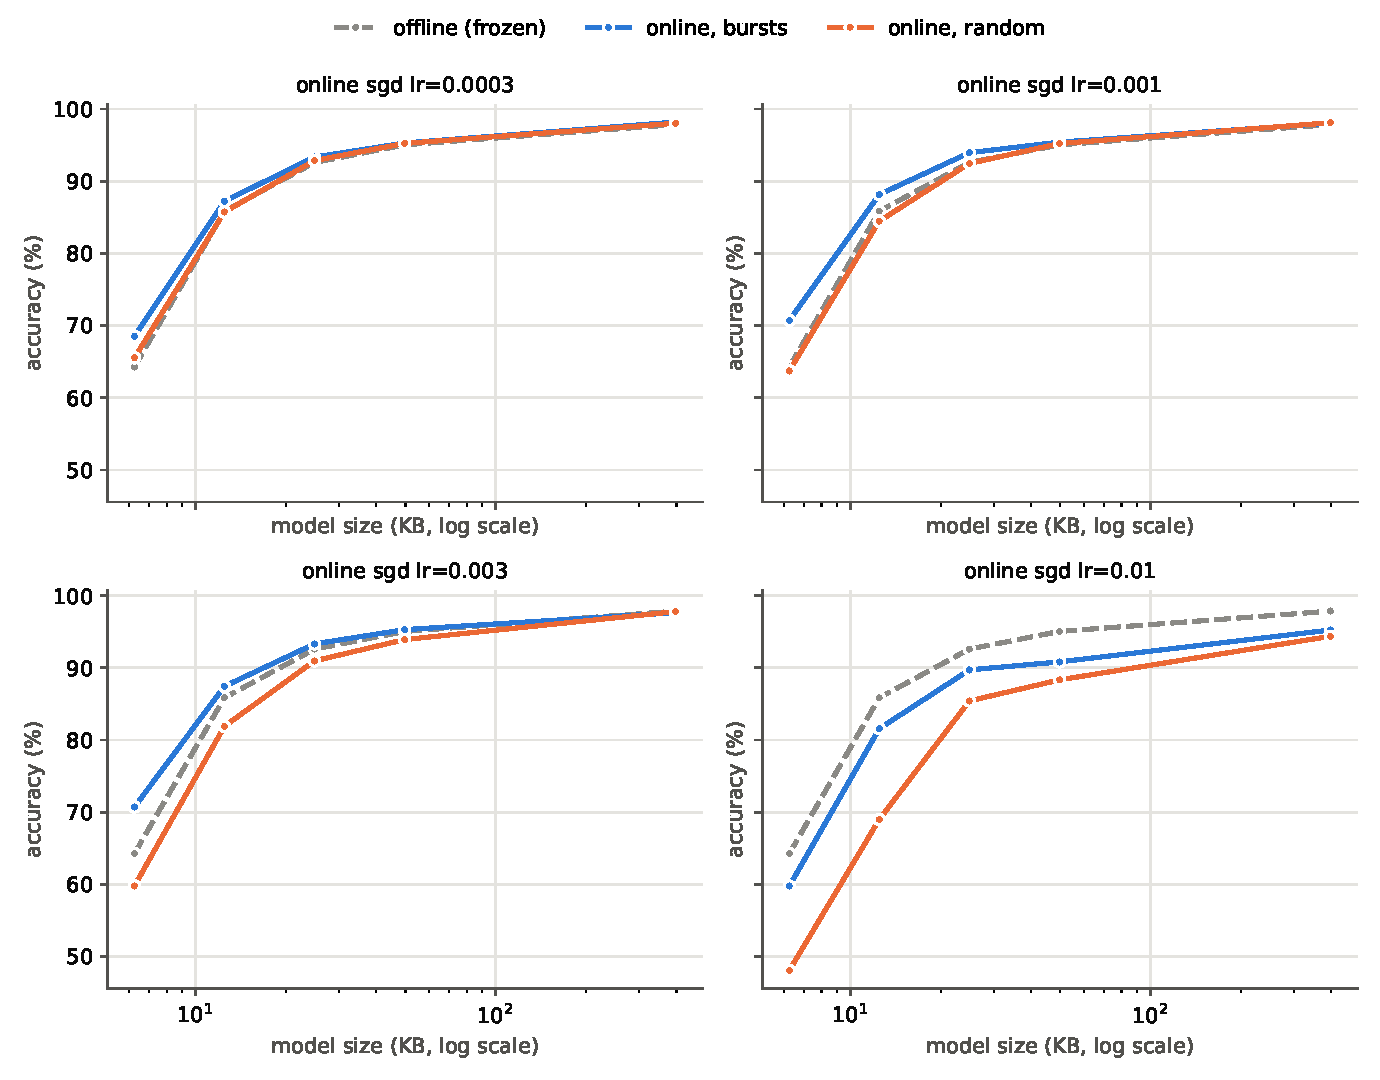
\includegraphics[width=0.7\linewidth]{figures/exp1_accuracy.pdf}
\caption{Experiment 1: accuracy against model size for the frozen model and the online model on each stream (online Adam, learning rate 0.001).}
\label{fig:exp1}
\end{figure}

The online model is always more accurate on the bursty stream than on the shuffled one, so there is a locality effect at every size.
It is small, between 0.3 and 1.3\,pp, and largest for $h=8$ and $h=4$.
However, online Adam lowers accuracy with respect to the frozen model at all sizes except $h=2$, where it is about equal.
The updates are too disruptive for the knowledge the models already have.

\subsection{Experiment 2: online learning rate}

The second experiment replaces Adam with plain SGD (no momentum) during the online phase and varies its learning rate: 0.0003, 0.001, 0.003 and 0.01.
The frozen models are the same as in Experiment~1, for $h \in \{128, 16, 8, 4, 2\}$.
Table~\ref{tab:exp2} gives the online gain and the locality effect; Figures~\ref{fig:exp2acc} and~\ref{fig:exp2loc} show them against model size.

\begin{table}[t]
\centering
\caption{Experiment 2: MLPs with online SGD at four learning rates. Online gain (bursts minus frozen) and locality effect (bursts minus random), in pp.}
\label{tab:exp2}
\begin{tabular}{rrr rrrr rrrr}
\toprule
 & & & \multicolumn{4}{c}{online gain} & \multicolumn{4}{c}{locality effect} \\
\cmidrule(lr){4-7} \cmidrule(lr){8-11}
$h$ & KB & frozen & 0.0003 & 0.001 & 0.003 & 0.01 & 0.0003 & 0.001 & 0.003 & 0.01 \\
\midrule
128 & 397.5 & 97.86 & $+0.33$ & $+0.19$ & $-0.22$ & $-2.35$ & $+0.16$ & $-0.05$ & $-0.15$ & $+1.13$ \\
16  &  49.7 & 95.04 & $+0.25$ & $+0.37$ & $+0.25$ & $-4.43$ & $+0.05$ & $+0.19$ & $+1.38$ & $+2.36$ \\
8   &  24.9 & 92.59 & $+0.75$ & $+1.36$ & $+0.72$ & $-2.87$ & $+0.48$ & $+1.49$ & $+2.35$ & $+4.31$ \\
4   &  12.5 & 85.85 & $+1.38$ & $+2.30$ & $+1.59$ & $-4.37$ & $+1.49$ & $+3.69$ & $+5.55$ & $+12.28$ \\
2   &   6.2 & 64.27 & $+4.25$ & $+6.44$ & $+6.45$ & $-4.50$ & $+2.98$ & $+6.99$ & $+10.93$ & $+11.69$ \\
\bottomrule
\end{tabular}
\end{table}

\begin{figure}[t]
\centering
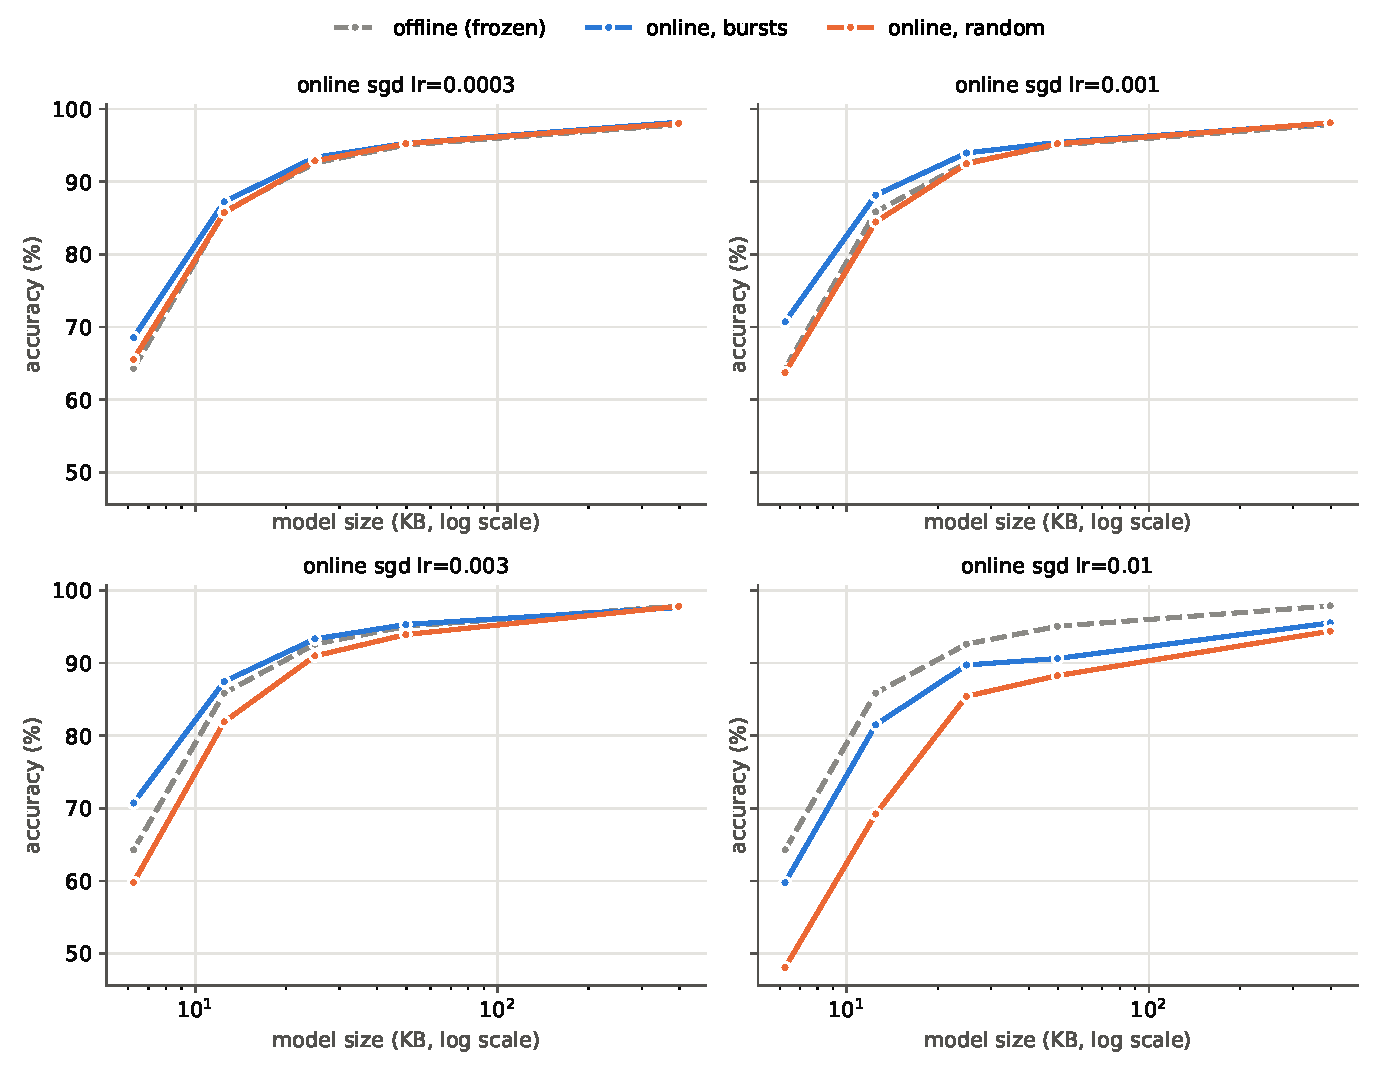
\includegraphics[width=\linewidth]{figures/exp2_accuracy.pdf}
\caption{Experiment 2: accuracy against model size, one panel per online learning rate.}
\label{fig:exp2acc}
\end{figure}

\begin{figure}[t]
\centering
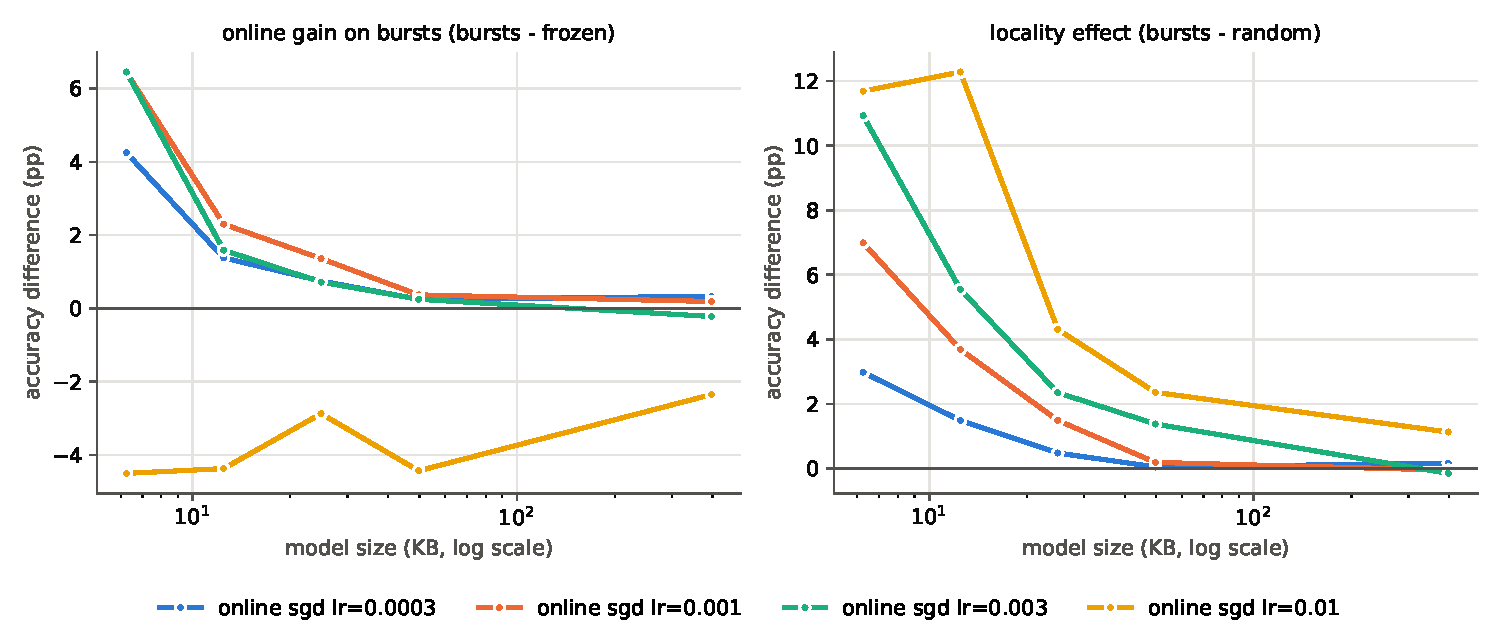
\includegraphics[width=\linewidth]{figures/exp2_locality.pdf}
\caption{Experiment 2: online gain (left) and locality effect (right) against model size, one line per online learning rate.}
\label{fig:exp2loc}
\end{figure}

With SGD and learning rates up to 0.003, online learning improves on the frozen model at almost every size.
The online gain grows as the model shrinks: below 0.4\,pp for $h \geq 16$, and above 6\,pp for $h=2$ at learning rates 0.001 and 0.003 (from 64.27\% to 70.71\% at 0.001).
On the shuffled stream the same small model gains little or loses accuracy (63.72\% at 0.001, 59.79\% at 0.003), so the gain comes from the order of the inputs and not from the extra training.

The locality effect grows in two directions: as the model gets smaller and as the learning rate gets larger.
At learning rate 0.01 it reaches 12.28\,pp for $h=4$, but there the online model is worse than the frozen one on both streams: the effect is large because accuracy on the shuffled stream collapses faster.
The best compromise between gain and stability lies between 0.001 and 0.003.

The large model ($h=128$) shows almost no locality effect at learning rates up to 0.003.
With enough capacity, the frozen model already covers the whole distribution and there is little to gain from adapting to the current context.

\subsection{Experiment 3: a small CNN}

The third experiment tests whether the effect appears in a small modern architecture.
Online learning uses SGD with learning rate 0.0003 and label smoothing 0.1.
Batch normalization raises a specific question in this setting: with a single image per step, the batch statistics are those of one image.

A first version updated the batch normalization statistics during the online steps.
It failed: online accuracy dropped below the frozen model at every width, by 6.9\,pp for $c=8$ and by 36.4\,pp for $c=4$ (from 94.36\% to 57.94\%), and the locality effect was negative for $c \leq 4$ (down to $-2.3$\,pp) and $+1.5$\,pp for $c=8$.
The final version keeps the batch normalization statistics frozen at their offline values and only trains the weights, including the scale and shift of the normalization layers.
Table~\ref{tab:exp3} and Figure~\ref{fig:exp3} show its results.

\begin{table}[t]
\centering
\caption{Experiment 3: CNNs with online SGD, learning rate 0.0003, batch normalization statistics frozen. Accuracy in \%, differences in pp.}
\label{tab:exp3}
\begin{tabular}{rrrrrrr}
\toprule
$c$ & KB & frozen & bursts & random & online gain & locality effect \\
\midrule
8 & 17.5 & 98.08 & 98.18 & 97.03 & $+0.10$ & $+1.15$ \\
4 &  4.8 & 94.36 & 93.27 & 89.76 & $-1.09$ & $+3.51$ \\
2 &  1.5 & 81.11 & 79.21 & 75.64 & $-1.90$ & $+3.57$ \\
1 &  0.5 & 42.14 & 31.35 & 13.14 & $-10.79$ & $+18.21$ \\
\bottomrule
\end{tabular}
\end{table}

\begin{figure}[t]
\centering
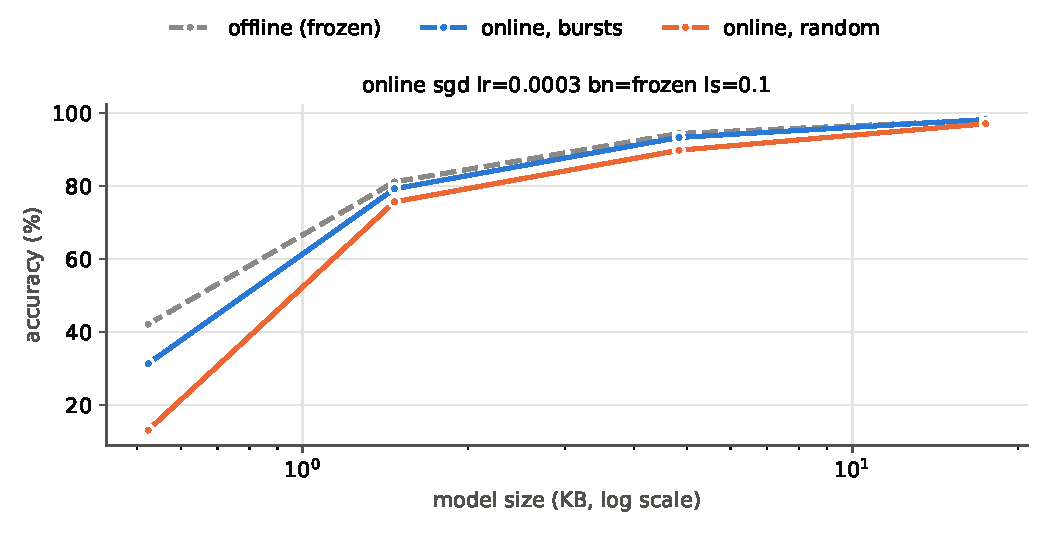
\includegraphics[width=0.7\linewidth]{figures/exp3_accuracy.pdf}
\caption{Experiment 3: accuracy against model size for the frozen CNN and the online CNN on each stream (online SGD, learning rate 0.0003, batch normalization statistics frozen).}
\label{fig:exp3}
\end{figure}

The CNN shows a locality effect at every width, and it grows as the model shrinks: from 1.15\,pp for $c=8$ to 3.5\,pp for $c=4$ and $c=2$, and 18.21\,pp for $c=1$.
However, online learning does not improve on the frozen model.
For $c=8$ the two are about equal (98.18\% against 98.08\%), and for smaller widths the online model is less accurate on both streams.
The smallest model ($c=1$, 0.5\,KB) is an extreme case: its frozen accuracy is only 42.14\%, and online learning lowers it to 31.35\% on bursts and to 13.14\% on the shuffled stream, close to chance.
The large locality effect at this width comes mostly from the collapse on the shuffled stream.

The CNN therefore behaves like the MLPs of Experiment~1 more than those of Experiment~2: the order of the inputs matters, but the updates cost more than they gain.
Only one online learning rate was tested.

\section{Discussion}

The experiments with MLPs support the hypothesis.
When capacity is very limited, a model that keeps adapting to the current context classifies a stream with temporal locality better than the same model frozen, and the advantage comes from the locality: it disappears or reverses on a shuffled copy of the stream.
The recency bias of online training, which hurts on the shuffled stream, helps on the bursty one.
Seen this way, the learning rate controls the length of the model's memory: a larger rate forgets faster and adapts faster.
The best value should depend on how long the contexts last, which here is about 50 images.

The results also have clear limits.
The task is MNIST and the stream is synthetic, with an idealized form of locality: bursts with sharp boundaries and only three classes each.
The online model receives the true label right after each prediction, which many applications cannot provide.
Every result comes from a single run with seed 0, so differences below about 0.5\,pp may not be meaningful.
The stream draws test images with replacement, so the online model sees some images more than once; the shuffled control has the same repetitions, and the locality effect cancels this out, but the online gain does not.
Finally, the CNN shows a locality effect, but no online gain at the only learning rate tested, so it is not yet clear whether the full result holds for convolutional networks.

\section{Conclusion and next steps}

Small MLPs trained online at inference time exploit the temporal locality of their input stream.
Below some model size they become more accurate than their frozen offline version, and the advantage is tied to the order of the inputs.
The effect grows as the model shrinks and as the online learning rate increases, up to the point where the updates become too disruptive.
A small CNN also benefits from the order of the inputs, but online learning did not make it more accurate than its frozen version.

Next steps include repeating the runs with several seeds, sweeping the online learning rate for the CNN as in Experiment~2, varying the burst length and the number of classes per burst, testing streams with natural locality (for example video), and replacing the true labels with weaker feedback.

\bibliographystyle{plainnat}
\bibliography{references}

\end{document}
